\chapter{Oefeningensessie 2}

\section{Oefening 6.3 p147}
Geef voor elk van de veranderlijken $a, b, c, d, e$ in het volgende programma aan of ze in het geheugen of in een register moeten bewaard worden, en waarom.
\begin{lstlisting}
int f(int a, int b){
	int c[3], d, e;
	d = a + 1;
	e = g(c, &b);
	return e + c[1] + b;
}
\end{lstlisting}
\begin{table}[ht]
	\centering
	\begin{tabular}{l | l | l}
		variabele & locatie & reden \\
		\hline
		$a$ & register & de variabele wordt enkel lokaal in de functie gebruikt\\
		$b$ & geheugen & het adres van b wordt opgevraagd en escapet dus de stack\\
		$c$ & geheugen & een array zit altijd in het geheugen\\
		$d$ & register & de variabele wordt enkel lokaal in de functie gebruikt\\
		$e$ & register & de variabele wordt enkel lokaal in de functie gebruikt\\
	\end{tabular}
\end{table}
\section{Oefening 8.6 p190}
Deel het volgende programma op in basisblokken.
\begin{lstlisting}
1	m := 0
2	v := 0
3	if v >= n: 	goto 15
4	r := v
5 	s := 0
6	if r < n: 	goto 9
7	v := v + 1
8	goto 3
9	x := M[r]
10	s := s + x
11	if s <= m:	goto 13
12	m := s
13	r := r + 1
14 	goto 6
15 	return m
\end{lstlisting}


\begin{figure}[ht]
	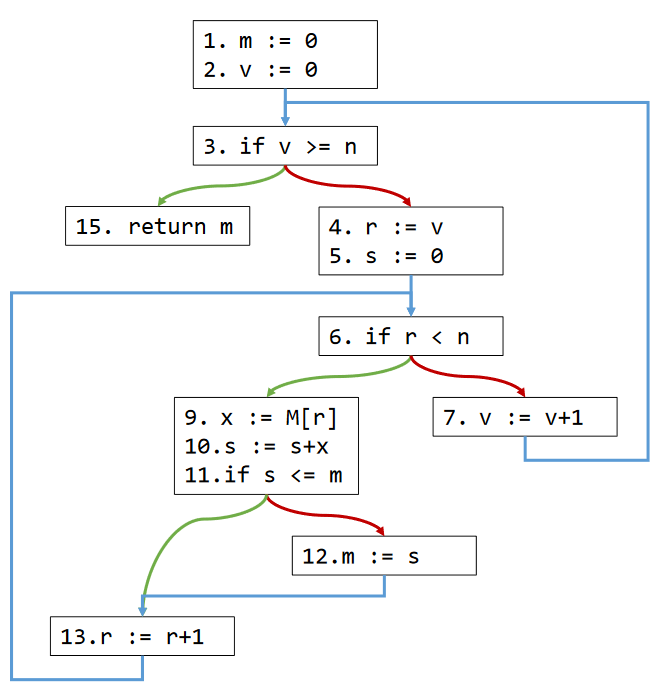
\includegraphics[width=\textwidth]{ex8_6p190}
\end{figure}

\section{Oefening 9.1 p217}
?